\chapter{Estado del Arte}\label{chapter:state-of-the-art}

\section{Sistemas, Modelos y Simulación}

Todo problema tiene un dominio en el cual se presenta y exige la construcción de un sistema, es decir, la selección y/o definición de entidades (mediante propiedades), relaciones estructurales y relaciones funcionales (entre estas entidades), las que se consideran involucradas y relevantes a la solución del problema. \parencite{temasdesimulacion} \\

Los sistemas se convierten en objeto de investigación para resolver el problema y se construyen y reconstruyen en varios niveles de abstracción según un proceso denominado modelación que suministra a diferentes niveles de abstracción representaciones estructurales y funcionales a las que se denomina modelos del sistema. El objetivo de crear modelos de un sistema tiene como fin esencialmente observar y/o modificar y/o controlar en condiciones ideales su conducta o dinámica. \parencite{temasdesimulacion} \\

La simulación es el proceso mediante el cual los procesos (dinámica) de un sistema son observados y/o modificados y controlados mediante modelos apropiados a tales fines. La dinámica de un sistema se considera simulada sólo en la medida en que esta dinámica, mediante su observación controlada, puede ser modificada con vistas a verificar principios o leyes y/o a determinar su forma más satisfactoria de realización. Siendo la computadora es el instrumento ideal para tales fines la simulación es esencialmente computacional. \parencite{temasdesimulacion} \\

De manera muy simple podemos decir que un sistema es  “[…] un conjunto de elementos relacionados entre sí y que funcionan como un todo”. \parencite{noauthor_simulacion_nodate} \\

\subsection{Sistema}

Según  \parencite{temasdesimulacion}, un sistema esta constituido por estructuras y procesos de un dominio de un problema las cuales se obtienen por abstracción a partir del dominio orientada por el problema.\\

A modo general existen varios tipos de sistemas, entre estos podemos mencionar los sistemas naturales, que están constituidos por estructuras y funciones de la realidad (átomos, partículas, sistemas biológicos); los sistemas socio-políticos, que son producto del desarrollo histórico, político y social (países, comunidades, sociedades); por último existen los denominados sistemas tecnológicos, resultado de la invención del hombre (máquinas, computadoras, sistemas eléctricos).\\

\subsubsection{Sistemas Dinámicos}

Los sistemas dinámicos son aquellos que tienen en cuenta el tiempo como dimensión fundamental y necesaria para describir su estructura, así como sus procesos. Existen dos tipos de sistemas dinámicos:
\begin{itemize}
	\item Sistema dinámico estacionario: la estructura del sistema no cambia y los procesos ocurren en el tiempo pero no se considera la dependencia del tiempo.
	\item Sistema dinámico no-e	stacionario: la estructura del sistema cambia con el tiempo y los procesos del sistema ocurren en y dependen del tiempo. \parencite{temasdesimulacion}
\end{itemize}

En esta investigación se trabajará con sistemas dinámicos a menos que el autor indique lo contrario.\\

\subsubsection{Sistema y Medio}

Un sistema existe (funciona, se desarrolla, interactúa) en un medio (ambiente). Medio es un sistema en el cual actúa, funciona, se desarrolla, con el cual interactúa en general un sistema bajo estudio. \parencite{temasdesimulacion}\\

Un sistema se considera cerrado si no se le asocia un medio, de lo contrario se le considera abierto. \parencite{temasdesimulacion}\\ Este se relaciona con su medio mediante entradas y salidas y a su vez este cambia en dependencia a su interacción con su medio.
No podemos dejar de mencionar el concepto de estado del sistema, que no es más que quien se encarga de almacenar lo mas importante de los estos cambios.
En general la acción del medio sobre un sistema (entrada) y el estado de este último son parámetros necesarios para predecir su comportamiento (estado) futuro y/o su salida o respuesta al medio. Luego, la dinámica de un sistema se describe en términos de una función de cambio de estado y una función de emisión de salida. \parencite{temasdesimulacion}\\

\subsubsection{Sistemas deterministas, no-deterministas y aleatorios}

Los sistemas se pueden distinguir en dependencia de la información que tengamos de estos, sea conocida, desconocida o parcialmente conocida (sistemas con información completa o incompleta).
Según lo anterior, un sistema se puede considerar determinista si los últimos estados de este se derivan de los anteriores o están determinados por ellos; por otra parte, se tienen los sistemas estocásticos o aleatorios en el que los estados futuros no están determinados por los anteriores.
Si un sistema es determinista, esto no implica necesariamente que los estados posteriores del sistema sean predecibles a partir del conocimiento de los anteriores. \parencite{darling_deterministic_nodate}

\subsection{Modelo}

Precisar cuáles entidades del sistema intervienen de algún modo en el problema que se desea resolver y las relaciones causales que influyen en su comportamiento y en el del sistema en su conjunto, conduce a un proceso de simplificación de la realidad, de abstracción, que se conoce como modelación.
Diferentes problemas sobre un mismo dominio da lugar a la concepción de diferentes sistemas sobre el mismo.\\

Los sistemas creados para solucionar un problema deben ser observables y/o controlables y/o modificables, o sea dado un sistema creado para resolver un problema se desea Observarlo y/o Controlarlo y/o Modificarlo. \parencite{temasdesimulacion}\\

Un modelo se utiliza para poder observar, controlar y modificar un sistema. Por lo tanto podemos definir un modelo como una descripción abstracta de un sistema que representa de forma aproximada su comportamiento.
Según \parencite{temasdesimulacion}, “Un modelo es un sistema que representa a otro sistema.”\\

Gran parte de los sistemas reales dificultan mucho que dicho modelo sea observable, controlable y modificable.\\

Podemos catalogar los modelos en dependencia de su estructura, entre estos tenemos los modelos del sistema real, a escala, analógico, matemático, computacional. En este último centraremos nuestra atención.\\

\subsubsection{Modelado Computacional}
El modelado computacional es el uso de computadoras para simular y estudiar sistemas complejos utilizando las matemáticas, la física y la informática. Un modelo computacional contiene numerosas variables que caracterizan el sistema bajo estudio. La simulación se realiza ajustando las variables, solas o combinadas, y observando los resultados. El modelado computacional permite a los científicos realizar miles de experimentos simulados por computadora. Los miles de experimentos por computadora identifican los pocos experimentos de laboratorio que tienen más probabilidades de resolver el problema bajo estudio. \parencite{noauthor_modelado_nodate}

Los modelos computacionales de hoy en día pueden estudiar sistemas muy complejos, y un caso particular de esto seria nuestro objeto de estudio, un \textbf{sistema de cultivos}, siendo este un sistema abierto, dinámico no estacionario, determinista en cierto punto con una gran porción de aleatoriedad e información la mayoría de veces incompleta. \\

\subsection{Simulación}
La simulación puede verse como la ejecución, observación y cambio de un modelo determinado.
Según la definición de Robert E. Shannon, \parencite{shannon1975simulacion} la simulación es el “[…] proceso de diseñar y desarrollar un modelo computarizado de un sistema o proceso y conducir experimentos con este modelo con el propósito de entender el comportamiento del sistema y/o evaluar varias estrategias con las cuales se puede operar el sistema”.\\

En las ciencias, la simulación es el artificio contextual que referencia la investigación de una hipótesis o un conjunto de hipótesis de trabajo utilizando modelos.
Simulación es una técnica numérica para conducir experimentos en una computadora digital. Estos experimentos comprenden ciertos tipos de relaciones matemáticas y lógicas, las cuales son necesarias para describir el comportamiento y la estructura de sistemas complejos del mundo real a través de largos periodos de tiempo. \parencite{noauthor_simulacion_nodate}\\

La simulación computacional es la basada en modelos computacionales.

Los recientes avances en las metodologías de simulación y la gran disponibilidad de diversos tipos de software existentes en el mercado han hecho que la técnica de simulación sea una de las herramientas más ampliamente usadas en el \textbf{análisis de sistemas}.

Gracias a los avances tecnológicos una computadora puede tomar el papel de cualquier máquina o sistema existente. A medida que aumenta la complejidad del sistema mas se dificulta para la computadora replicar dicho comportamiento, por lo tanto es necesario emplear modelos del sistema simplificado, tomando solo de este lo que sea relevante para el análisis.

\subsubsection{Modelado de sistemas complejos}

En la actualidad, debido a los avances tecnológicos del microprocesador, han nacido nuevas técnicas de modelado de sistemas complejos, entre estas podemos mencionar dos grandes exponentes que son la simulación basada en agentes y la dinámica de sistemas. Ambas complementan modelos no formales de sistemas complejos y modelos matemáticos con un mayor nivel de abstracción.\\

Varios filósofos como Hesse \parencite{echenique1970models} y Hughes \parencite{hughes1997models} proponen un esquema general del proceso científico. Estos modelos se construyen para desarrollar procesos de inferencia sobres algunos aspectos de sistemas reales observados con anterioridad. Tomando como base estos procesos de inferencia se mejora la forma de entender los sistemas reales observados. \parencite{izquierdo2008modelado}

En la figura (\ref{fig:img_1}) se muestra el proceso de creación y uso de un modelo.

\begin{figure}[!h]
	\centering
	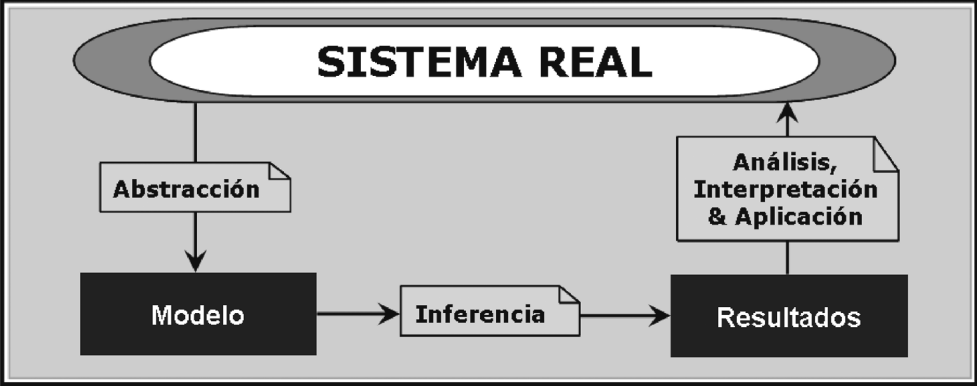
\includegraphics[scale=0.5]{Images/esquema_modelado_cientifico.png}
	\caption{Esquema general del proceso de modelado científico. \parencite{izquierdo2008modelado}}
	\label{fig:img_1}
\end{figure}

Se puede concluir que luego de analizar un modelo, se llegaran a conclusiones que no serán estrictamente rigurosas respecto a lo que sucede en el sistema real. Sin embargo, con la aplicación del modelo se obtendrán conocimientos que sin esta no hubiese sido posible adquirir.\\

Como se observa en la figura (\ref{fig:img_1}), el proceso de modelado no es unidireccional ya que generalmente se suele diseñar un modelo, del cual se obtienen resultados, teniendo en cuenta estos se perfecciona el modelo mediante ciertos cambios lógicos en sus valores iniciales o intermedios. El modelo inicial puede haber fallado por dos motivos fundamentales:
\begin{itemize}
	\item porque no parecieran derivarse lógicamente de las premisas del modelo (proceso de verificación).
	\item porque, aún siendo lógicamente correctos, difirieran excesivamente de los resultados observados en el sistema real que se está modelando (proceso de validación). \parencite{izquierdo2008modelado}
\end{itemize}

De una manera un tanto informal, podríamos decir que verificar consiste en valorar si el modelo que tenemos es correcto, mientras que validar consiste en estudiar si tenemos el modelo correcto.\\


Los sistemas complejos (p. ej. organismos pluricelulares, colonias de hormigas, ecosistemas, economías, sociedades…) están caracterizados por tener una estructura compuesta por varios niveles. En estos sistemas complejos \parencite{vicsek2002complexity, gilbert2004agent}:

\begin{itemize}
	\item Los componentes de niveles jerárquicos inferiores suelen mostrar un grado de autonomía significativo.
	\item El comportamiento del sistema surge a partir de la auto-organización de sus componentes, sin que esta organización esté controlada ni dirigida por ningún ente exterior al sistema.
	\item Los componentes básicos de estos sistemas complejos (células, hormigas, individuos, poblaciones, empresas…) perciben su entorno y responden a cambios en él de forma potencialmente diferente.
\end{itemize}

Todas estas características hacen que el proceso de modelado formal de sistemas complejos difiera sustancialmente del de otros sistemas más simples. En particular, su naturaleza descentralizada, la presencia de bucles de causalidad y retroalimentación no lineales, y el hecho de contener varias unidades más o menos autónomas, que pueden interaccionar, evolucionar, y adaptar su comportamiento a cambios en el entorno, implica que en la mayoría de los casos es muy difícil —si no imposible— conseguir un modelo que pueda describir el sistema complejo adecuadamente y que además sea resoluble matemáticamente. \parencite{izquierdo2008modelado}\\

Un modelo computacional es un modelo formal (que por lo tanto puede expresarse en lenguaje matemático como un conjunto de ecuaciones), y la simulación computacional es una herramienta que nos permite estudiarlo más allá de los límites actuales de las matemáticas. De este modo, el resultado final es un modelo potencialmente más realista, y que todavía conserva el rigor formal de los modelos matemáticos más tradicionales. \parencite{izquierdo2008modelado}\\

Luego de analizada la posibilidad de trabajar con modelos formales de mayor complejidad, se hace necesario ampliar el esquema visto en la figura (\ref{fig:img_1}) a la siguiente (\ref{fig:img_2}):

\begin{figure}[!h]
	\centering
	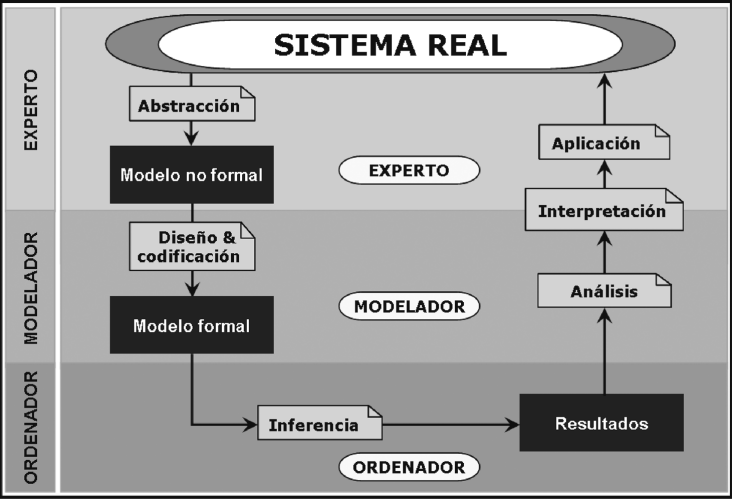
\includegraphics[scale=0.5]{Images/esquema_modelado_cientifico_con_abstraccion.png}
	\caption{Proceso de modelado con abstracción intermedia. \parencite{izquierdo2008modelado}}
	\label{fig:img_2}
\end{figure}

\subsubsection{Simulación basada en agentes}

La simulación basada en agentes (agent-based modelling) es un novedoso método de investigación para las ciencias sociales. Dicho método fue inicialmente desarrollado en el campo de la IA (Inteligencia Artificial) a lo largo de la década de los 50 del pasado siglo y ha sido empleado desde entonces para resolver algunos de los problemas propios de las ciencias físicas y naturales. Sin embargo, ha empezado a utilizarse recientemente en las ciencias sociales, aunque su objeto de estudio difiera de los de las ciencias físicas y naturales. \parencite{garcia2016simulacion}\\

Mediante la simulación basada en agentes, el modelador reconoce
explícitamente que los sistemas complejos, y en particular los sociales, son
producto de comportamientos individuales y de sus interacciones. \parencite{izquierdo2008modelado}
Este tipo de simulación se distingue de de otras por la forma en que se construye la primera abstracción del sistema real y por tanto del modelo formal.\\

Se caracterizan por comprender varios agentes que son, en mayor o menor grado, autónomos, heterogéneos e independientes, que muestran cada uno sus propias metas y objetivos, y que generalmente son capaces de interaccionar entre sí y con su entorno \parencite{torsun1995foundations}. En muchas ocasiones, pero no siempre, son sistemas caracterizados por la existencia de un número grande de agentes relativamente simples, que pueden evolucionar a lo largo del tiempo para adaptarse a nuevas condiciones del entorno o a nuevos objetivos. \parencite{izquierdo2008modelado}

A continuación se pueden ver los cuatro tipos básicos de agentes encontrados en casi todos los sistemas inteligentes:
\begin{itemize}
	\item Agentes reactivos simples: son el tipo de agente más sencillo. Estos agentes seleccionan las acciones sobre la base de las percepciones actuales, ignorando el resto de las percepciones históricas.
	\item Agentes reactivos basados en modelos: La forma más efectiva que tienen los agentes de manejar la visibilidad parcial es almacenar información de las partes del mundo que no pueden ver. O lo que es lo mismo, el agente debe mantener algún tipo de estado interno que dependa de la historia percibida y que de ese modo refleje por lo menos alguno de los aspectos no observables del estado actual.
	\item Agentes basados en objetivos: El conocimiento sobre el estado actual del mundo no es siempre suficiente para decidir qué hacer. En otras palabras, además de la descripción del estado actual, el agente necesita algún tipo de información sobre su meta que describa las situaciones que son deseables.
	\item Agentes basados en utilidad: Las metas por sí solas no son realmente suficientes para generar comportamiento de gran calidad en la mayoría de los entornos. Las metas sólo proporcionan una cruda distinción binaria entre los estados de «felicidad» y «tristeza», mientras que una medida de eficiencia más general debería permitir una comparación entre estados del mundo diferentes de acuerdo al nivel exacto de felicidad que el agente alcance cuando se llegue a un estado u otro. Como el término «felicidad» no suena muy científico, la terminología tradicional utilizada en estos casos para indicar que se prefiere un estado del mundo a otro es que un estado tiene más utilidad que otro para el agente. \parencite{russell2004inteligencia}
\end{itemize}
Puesto que el énfasis en la simulación basada en agentes está en encontrar abstracciones apropiadas que describan los componentes básicos del sistema y sus interacciones (en vez de buscar abstracciones que versen directamente sobre la dinámica global del sistema), esta técnica de modelado es particularmente útil para modelar procesos emergentes de forma natural.\parencite{izquierdo2008modelado}

\subsubsection{Simulación basada en dinámica de sistemas}































